\section{Outerplanar and Hamiltonian graphs}
Zoltán Lóránt Nagy \cite{outerplanar} showed that the conjecture of Goddard and Henning holds for
Hamiltonian graphs. For this, he characterized the $2$-coupon colorable
maximal outerplanar graphs first.

\begin{definition}
   A graph is outerplanar if it has a planar drawing for which all vertices
   belong to the outer face. A maximal outerplanar graph is a simple outerplanar graph
   such that adding any edge results in a non-outerplanar graph.
\end{definition}
\begin{remark}
  The outer face of a maximal outerplanar graph is a Hamiltonian cycle.
\end{remark}

In order to provide the mentioned characterization we need to introduce a few
notions first.
\begin{definition}
  Let $G$ be a maximal outerplanar graph of order $n \ge 3$. The $M(G)$ sun graph
  of $G$ is obtained by gluing a triangle to each edge of the outer face.
\end{definition}
\begin{remark}
  $M(G)$ is a maximal outerplanar graph with $2n$ vertices, from which $n$ has
  degree $2$.
\end{remark}
\begin{remark}
  If $G$ has an odd number of vertices, then $M(G)$ does not have two disjoint
  total dominating sets, as in a $2$-coupon coloring of $M(G)$ the vertices of
  $G$ must have alternating colors. The graph on figure $\ref{fig:sungraph}$ is
  the sun graph of the $BDE$ triangle.
\end{remark}
\begin{definition}
  A vertex $v$ of a maximal outerplanar graph is called a central vertex if the
  following $3$ conditions hold.
  \begin{enumerate}
    \item $deg(v) \ge 3$
    \item Every neighbor of $v$ has degree at least $3$.
    \item For every $u, w$ neighbors of $v$ the length of the $uw$ path on the
    outer face not containing $v$ is divisible by $4$.
  \end{enumerate}
\end{definition}
\begin{claim}
  The outer face of a maximal outerplanar graph does not contain two consecutive
  central vertices.
\end{claim}
\begin{proof}
  Suppose there exists an $uv$ edge on the outer face such that $u$ and $v$ are
  central vertices. Because of the maximality of the graph there exists a $uvw$
  triangle. Index the vertices along the outer face form $v = v_1$ to $u = v_{n}$.
  Suppose $w = v_i$. From the centrality of $v$ follows that $i \equiv 2\
  (\textrm{mod}\ 4)$. On the other hand, $u$ is also a central vertex, hence
  $i \equiv 1\ (\textrm{mod}\ 4)$.
\end{proof}
\begin{definition}
  A generalized sun graph is a maximal outerplanar graph of order
  $n \equiv 2\ (\textrm{mod}\ 4)$ such that the number of
  degree $2$ vertices plus the number of central vertices is $n/2$.
\end{definition}
\begin{remark}
  Every second vertex of the outer face in a generalized sun graph is either
  central or has degree $2$.
\end{remark}

The key characterization theorem is the following.

\begin{thm}\label{thm:outerplanar}
  Let $G$ be a maximal outerplanar graph of order at least $4$. $G$ admits $2$ disjoint total dominating
  sets if and only if $G$ is not a generalized sun graph.
\end{thm}

For proving this theorem we need some observations about generalized sun graphs.

\begin{definition}
  Let $G$ be a maximal outerplanar graph and $i \ge 2$. We say that a $uv$ edge is a chord
  of length $i$, if there is a $uv$ path of length $i$ on the outer face. (This means
  that if $uv$ is a chord of length $i$, then it is also a chord of length $n - i$.)
\end{definition}

\begin{lemma} \label{lem:two_chord}
  A maximal outerplanar graph of order $n \ge 3$ has a chord of length $2$.
\end{lemma}
\begin{proof}
  It is trivial for $n = 3$. Suppose $n \ge 4$ and
  let $uv$ be a chord of minimal length. By
  the maximality of the graph there exists a $uvw$ face, where $w$ is on the shorter
  $uv$ path of the outer face. If $uv$ is not a chord of length $2$, then $uw$ or $vw$
  is a chord of length less than the length of the $uv$ chord.
\end{proof}

\begin{lemma} \label{lem:3-4_chord}
  A maximal outerplanar graph of order $n \ge 5$ has a chord of length $3$ or $4$.
\end{lemma}
\begin{proof}
  Let $uv$ be a chord of minimal length among chords of length at least $3$. By
  the maximality of the graph there exists a $uvw$ face, where $w$ is on the $uv$ path
  on the outer face that defines the length of the chord. If on this path $w$ has a distance
  bigger than $2$ from either $u$ or $v$, than $uw$ or $vw$ is a chord contradicting
  the minimality of $uv$. Thus, the length of the $uv$ path is at most $4$.
\end{proof}

\begin{lemma} \label{lem:del_face}
  If $G$ is a maximal planar graph of order $n \ge 7$, then there exists a bounded
  face, such that the deletion of this face divides $G$ into three graphs with the
  following properties.
  \begin{enumerate}
    \item At most one of the three graphs has more than $3$ bounded faces.
    \item At least one of the three graphs has $2$ or $3$ faces.
  \end{enumerate}
\end{lemma}
\begin{proof}
  For $n \le 11$, the statement is easy to verify.

  For $n > 11$ delete the faces with $2$ common edges with the unbounded face. Then in the remaining
  graph $G_1$ delete the faces that now have $2$ common edges with the unbounded face.

  We claim that the remaining graph $G_2$ is not empty. $G$
  has $m = \frac{3(f - 1) + n}{2}$ edges, where $f$ denotes the number of faces.
  Then by Euler's formula $n = f + 1$, hence $G$ has at least $11$ faces. In the
  first deleting step at most $n/2$ faces are deleted, and in the second step at most
  $|G_1|/2$ faces are deleted. Thus at most $3(f + 1) / 4$ faces are deleted.
  $3(f + 1) / 4 \le f - 2$ if $f \ge 11$.

  Finally, choose a face $f_0$ from the remaining graph $G_2$, that has $2$ common edges with
  the unbounded face of $G_2$. We claim that $f_0$ has the desired properties. $f_0$ has at most
  one neighboring face in $G_2$, and one or two neighboring faces $f_1$ and maybe $f_2$ outside of $G_2$.
  Both of $f_1$ and $f_2$ has at most two neighboring faces outside of $G_1$, and
  at least one of $f_1$ and $f_2$ has at least one neighboring face outside of $G_1$.
\end{proof}

\begin{proof}[Proof of Theorem \ref{thm:outerplanar}]
  First we show that generalized sun graphs do not have $2$ disjoint total
  dominating sets. The proof goes by induction on the $n = 4k + 2$ number of vertices.

  For $k = 1$ there is only one generalized sun graph and it does not admit $2$
  disjoint total dominating sets. (Shown on figure \ref{fig:sungraph}.)

  Suppose $k \ge 2$ and $G$ is a generalized sun graph of order $4k + 2$. Index
  the vertices along the outer face from $v_1$ to $v_{4k + 2}$, such that every
  vertex with an odd index is central or has degree $2$. Let $c$ be a $2$-coloring of
  the graph. We show that $c$ cannot be a $2$-coupon coloring. The cardinality of the
  vertices implies that there must be two consecutive vertices $v_{2i}$ and $v_{2i + 2}$
  with the same color (say white). If $v_{2i + 1}$ has only white neighbors, then this
  coloring is not a $2$-coupon coloring. So suppose $v_{2i + 1}$ has a black neighbor
  $v_j$. In this case $v_{2i + 1}$ is a central vertex. The $v_{2i + 1}v_j$ edge divides the graph
  into two parts ($v_{2i + 1}v_j$ is an edge in both graphs). Both of
  these graphs are generalized sun graphs, as $v_{2i + 1}$ either remains a central
  vertex or becomes a vertex of degree $2$ in these smaller graphs, whereas other
  central vertices remain central vertices. By induction, the restriction of
  $c$ is not a $2$-coupon coloring in either of the smaller graphs. If there is
  a vertex $v_l$ with a monochromatic neighborhood in one of the smaller graphs
  and $l \neq 2i + 1,\ l \neq j$, then $v_l$ has the same neighborhood in $G$, hence
  all its neighbors are from the same color class. $v_{2i + 1}$ cannot violate the
  condition, as it was chosen in a way that it has both a black and a white neighbor
  in both graphs. Thus the only remaining case is when $v_j$ has a monochromatic
  neighborhood in both graphs. But in this case all of its neighbors are from
  the same color class as $v_{2i + 1}$, so it has a monochromatic neighborhood also
  in $G$.

  \vspace{0.4cm}

  Now we show that if a graph $G$ of order $n$ is not a generalized sun graph
  then it does have two disjoint total dominating sets.

  If $n \equiv 0\ (\textrm{mod}\ 4)$, then it is easy to find a $2$-coupon coloring:
  color the vertices along the boundary of the outer face by repeating the pattern
  $BBWW$.

  If $n \equiv 1\ (\textrm{mod}\ 4)$, then the same coloring method works, if you
  start the coloring from the right vertex. By lemma \ref{lem:two_chord} there
  exists a chord $uv$ of length $2$. Alternating colors in pairs starting from $v$
  does the job. (See Figure \ref{fig:4k+1}.)
  \begin{figure}[h]
    \centering
    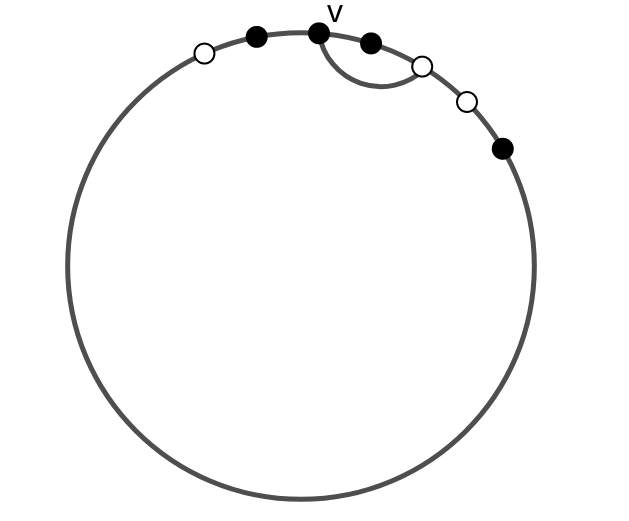
\includegraphics[width=50mm]{4k+1}
    \caption{Coloring an outerplanar graph of order $4k + 1$}
    \label{fig:4k+1}
  \end{figure}

  If $n \equiv 3\ (\textrm{mod}\ 4)$, then start the coloring from a vertex next
  to $v$. (See Figure \ref{fig:4k+3}.)
  \begin{figure}[h]
    \centering
    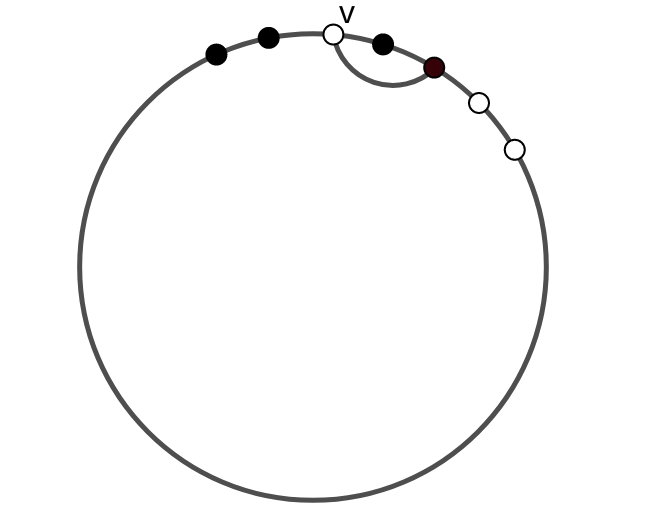
\includegraphics[width=50mm]{4k+3}
    \caption{Coloring an outerplanar graph of order $4k + 3$}
    \label{fig:4k+3}
  \end{figure}

  Suppose $n \equiv 2\ (\textrm{mod}\ 4)$. We show by induction that if $G$ does not have $2$
  disjoint total dominating sets, then it is a generalized sun graph.\\
  The case $k = 1$ is easy to check.\\
  If $G$ has a chord $uv$ of length $3$, then $uv$ divides the graph into two parts:
  $G_1$ of order $4$ and $G_2$ of order $4k$. By alternating colors in pairs one can obtain
  $2$-coupon colorings of $G_1$ and $G_2$, where both $u$ and $v$ are colored to black
  in both graphs.\\
  If $G$ does not have a chord of length $3$, then by Lemma \ref{lem:3-4_chord}
  there exists a chord $uv$ of length $4$. Then $uv$ divides $G$ into two graphs.
  One of them must be the maximal outerplanar graph $G_5$ of order $5$. $u$ and $v$
  must be the degree $3$ vertices of $G_5$, as otherwise there would be a chord of length $3$
  in $G$. Note that in a $2$-coupon coloring $u$ and $v$ must have the same colors
  in order to create a proper neighborhood for the degree $2$ vertices of $G_5$.
  Consider the face $uvw$, where $w$ is not in $G_5$. The deletion of this face
  divides $G$ into $3$ graphs: $G'$, $G''$ and $G_5$. (It might be that $G'$ or $G''$ is
  degenerated in the sense that it consists only of one edge.) Let $G'$ be the graph containing
  $u$ and $w$. Without loss of generality we may assume that $|G''| \le |G'|$.\\
  Choose the $uv$ chord in a way, such that $|G'|$ is minimal. We may assume that
  $G'$ has at most $3$ faces by Lemma \ref{lem:del_face}, and thus $|G'| \le 5$.
  Thus, there are $4$ cases depending on the size of $G'$.

  \begin{itemize}
    \item Case $1$: $|G'| = 2$.
      In this case $G''| = 4k - 2$. If $G''$ has a $2$-coupon coloring, then
      it can easily be expanded to a $2$-coupon coloring of $G$. If $G''$ does
      not have a $2$-coupon coloring, then it is a generalized sun graph by induction.
      If $v$ is a degree $2$ or central vertex in $G''$, then color the vertices of $G''$ by
      alternating colors in pairs, starting with white from $w$, but color $v$ to
      black. Let $x$ denote the vertex before $v$. (See Figure \ref{fig:case1}.)
      \begin{figure}[h]
        \centering
        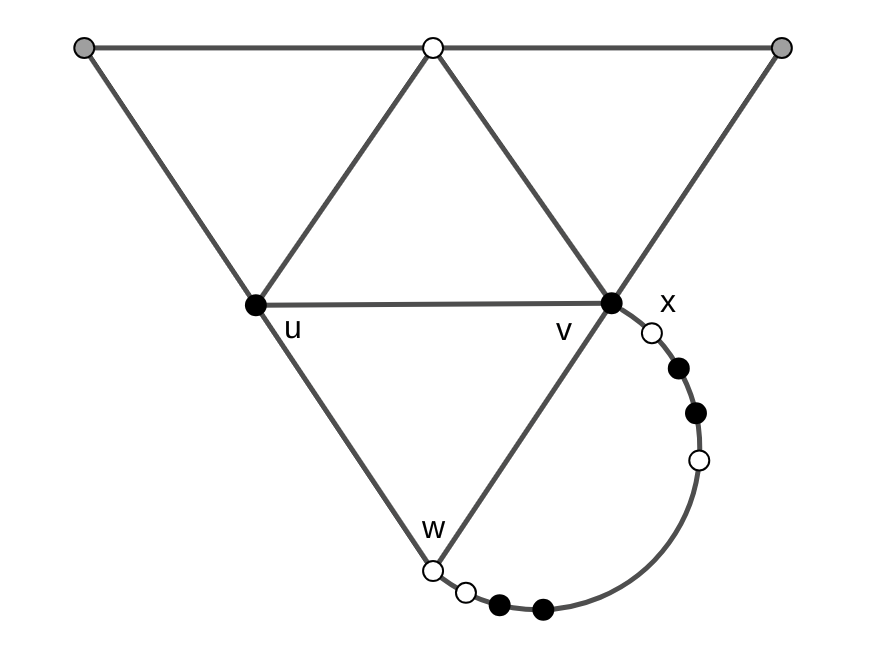
\includegraphics[width=60mm]{case1}
        \caption{Case $1$}
        \label{fig:case1}
      \end{figure}
      This way, only $v$ can have a monochromatic neighborhood in $G''$: if $v$ has degree
      $2$, then $wx$ is an edge, and if $v$ is central, then $v$ and $x$ have a common
      neighbor in $G''$ and $v$ has only white neighbors. $G_5$ can be colored to
      provide $v$ the missing color. \\

      If $v$ is neither a degree $2$ vertex nor a central vertex, then $w$ is. In
      this case $w$ is a central vertex in $G$ and thus $G$ is a generalized sun graph.
    \item Case 2: $|G'| = 3$.
      In a $2$-coupon coloring $u$ and $v$ must have the same color, whereas $u$
      and $w$ must have different colors. Let $H$ be the graph obtained from $G$
      by deleting $G_5$ and identifying $uw$ with $vw$. (See \ref{fig:case2})
      $G$ is $2$-coupon colorable if and only if $H$ is $2$-coupon colorable. On the other hand,
      $G$ is a generalized sun graph if and only if $H$ is a generalized sun graph.
      \begin{figure}[h]
        \centering
        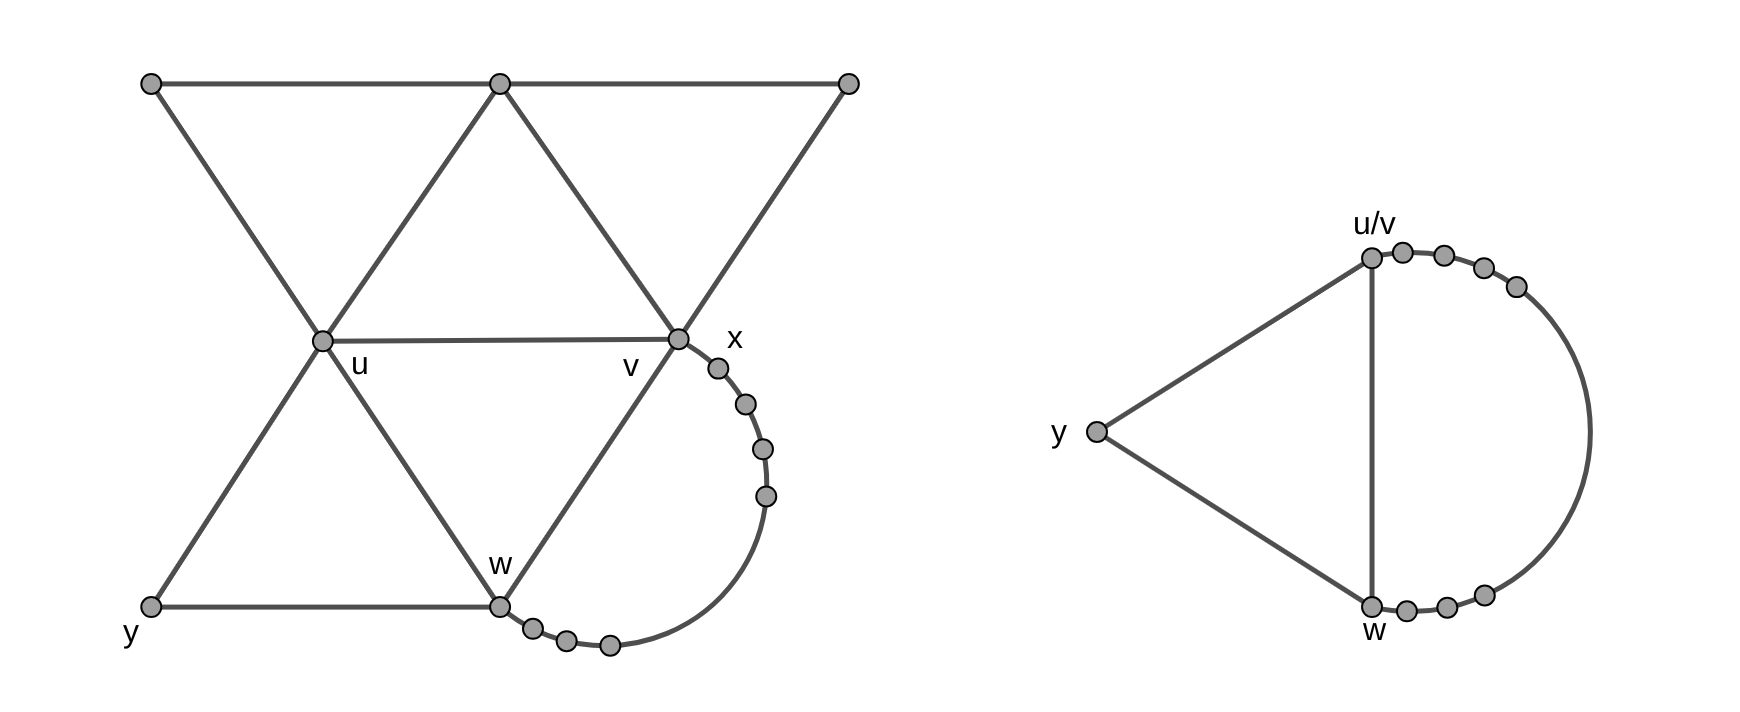
\includegraphics[width=150mm]{case2}
        \caption{Case $2$: $G$ (left) and $H$ (right)}
        \label{fig:case2}
      \end{figure}
    \item Case $3$: $|G'| = 4$.
      If $|G'| = 4$, then $uw$ is a chord of length $3$, and that is a contradiction.
    \item Case $4$: $|G'| = 5$.
      $u$ and $w$ must be the degree $3$ vertices in $G'$, otherwise we could
      find a chord of length $3$. In a $2$-coupon coloring $u$ and $w$ must have
      the same color. Let $H$ be the graph obtained from $G$ by deleting $G_5$
      and identifying $uw$ with $vw$. (See \ref{fig:case4})
      \begin{figure}[h]
        \centering
        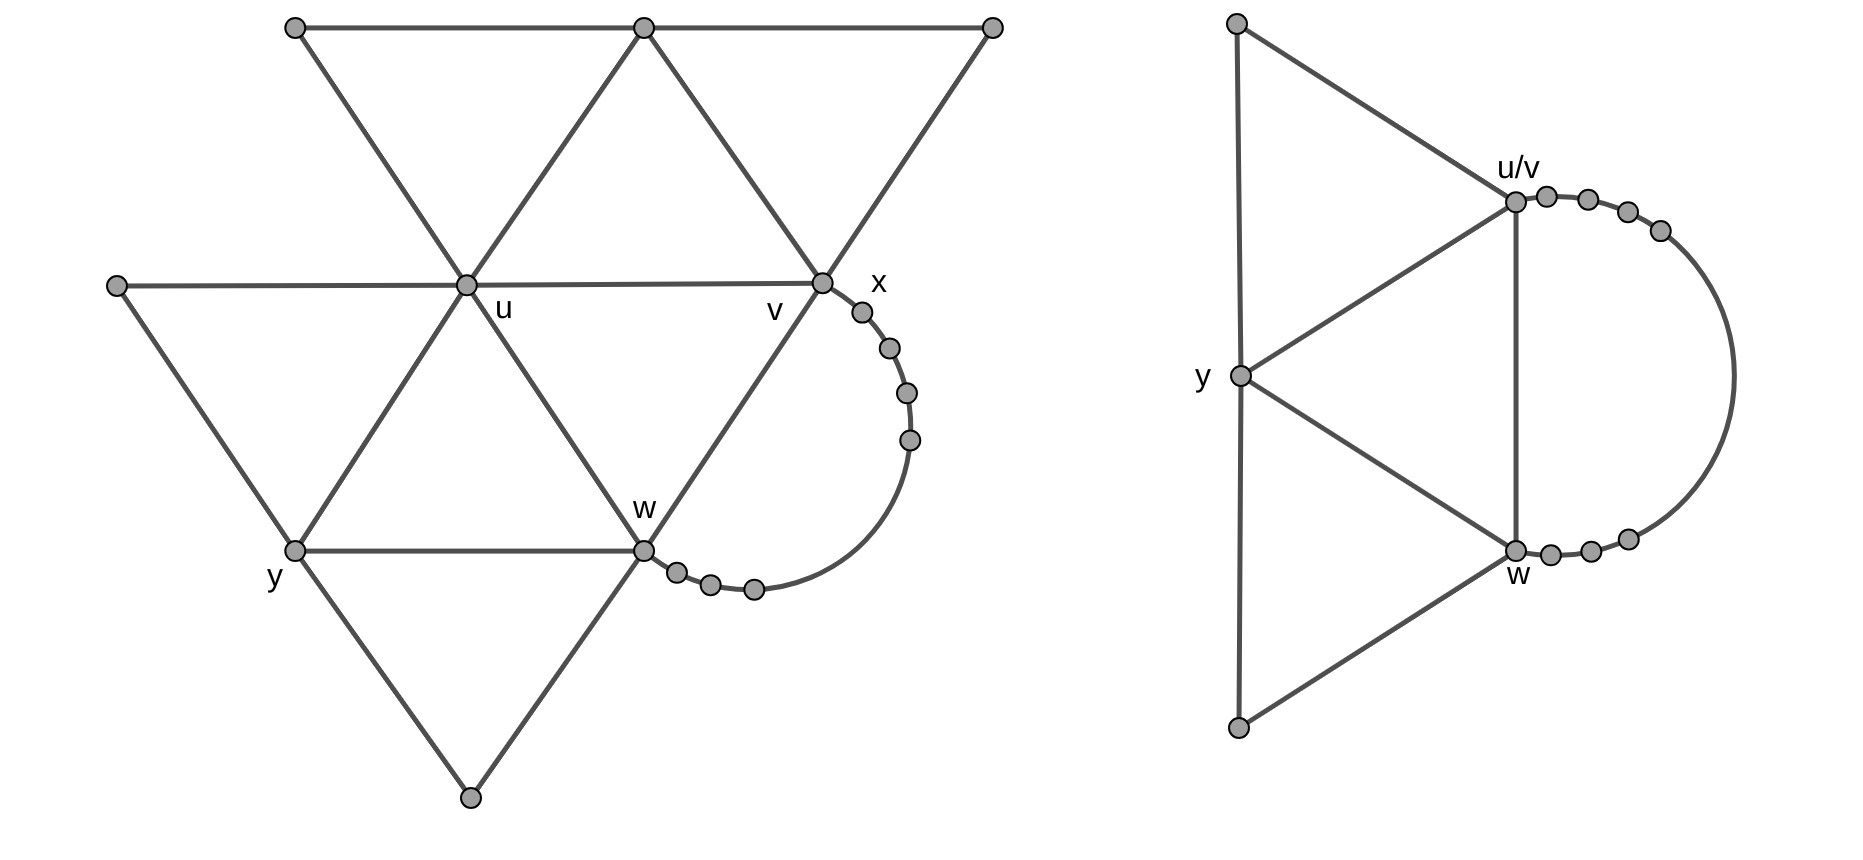
\includegraphics[width=150mm]{case4}
        \caption{Case $4$: $G$ (left) and $H$ (right)}
        \label{fig:case4}
      \end{figure}
      $G$ is $2$-coupon colorable if and only if $H$ is $2$-coupon colorable. On the other hand,
      $G$ is a generalized sun graph if and only if $H$ is a generalized sun graph.
  \end{itemize}
\end{proof}

\begin{remark}
  With a slight modification of the proof it can be shown that the vertices of a
  generalized sun graph cannot be colored in a way that every degree $2$ or central
  vertex has neighbors from both color classes.
\end{remark}

As mentioned earlier, based on this theorem Zoltán Lóránt Nagy \cite{outerplanar}
also showed that the total dominating number of Hamiltonian triangulated graphs
is at least two. We still need a Lemma for proceeding with the proof.

\begin{lemma}\label{lem:central}
  If $G$ is a generalized sun graph of order $4k + 2$, then there exist at most
  $k - 1$ chords incident to a central vertex.
\end{lemma}
\begin{proof}
  The proof goes by induction. If $k = 1$, then there exists only one generalized sun graph
  of order $4k + 2$, and it does not have any central vertices. Suppose $k > 1$.
  We are done, if there is no chord incident to a central vertex. Otherwise, let $uv$ be
  such a chord of minimal length, where $v$ is central. $uv$ divides the graph into
  two generalized sun graphs. In both of these graphs, $v$ is either a degree $2$
  vertex or a central vertex. Hence all the chords incident to a central vertex in $G$
  must be either $uv$ or a chord with the same property in one of the smaller graphs.
  By the minimality of $uv$, one of these graphs does not have chords incident to
  a central vertex. The other graph is of order at most $4(k - 1) + 2$, thus by induction
  it contains at most $k - 2$ chords incident to a central vertex.
\end{proof}

\begin{cor} \label{col:degree2}
  In a generalized sun graph the number of central vertices is less than the number
  of degree $2$ vertices.
\end{cor}
\begin{proof}
  Let $G$ be a generalized sun graph of order $4k + 2$. The number of central
  vertices is at most $k - 1$ by the previous lemma. The number of degree $2$ or
  central vertices is $2k + 1$.
\end{proof}

\begin{thm} \label{thm:ham}
  Every triangulated graph with a Hamiltonian circle admits $2$ disjoint
  dominating sets.
\end{thm}
\begin{proof}
  A Hamiltonian triangulated graph $G$ can be obtained by identifying the Hamiltonian cycle
  of two maximal outerplanar graphs $G_1$ and $G_2$. If at least one of these outerplanar graphs is
  $2$-coupon colorable, then the same coloring is a $2$-coupon coloring of $G$.
  By Theorem \ref{thm:outerplanar} we are done if at least one of these graphs is
  not a generalized sun graph.

  Suppose that $G_1$ and $G_2$ are generalized sun graphs. If the union of degree
  $2$ vertices and central vertices is the same in $G_1$ and $G_2$, then by Corollary
  \ref{col:degree2} there exists a vertex with degree $2$ in both graphs. Then this
  vertex is a degree $2$ vertex in $G$ and that is a contradiction, as in a triangulated
  planar graph every degree must be at least $3$.

  Assume that each vertex is a degree $2$ or central vertex in $G_1$ or $G_2$.
  Index the vertices along the Hamiltonian cycle from $v_1$ to $v_{4k + 2}$.
  We claim that there exists an index $i$ such that $v_i$ is a degree $2$ vertex
  in $G_1$ and $v_{i + 3}$ is a degree $2$ vertex in $G_2$. (If $i + 3$ is bigger than
  $4k + 2$, we take $v_{i + 3 - (4k + 2)}$.) Let $I_1 = \{i | deg_{G_1}(v_i) = 2\}$,
  $I_2 = \{i | deg_{G_2}(v_i) = 2\}$ and $J = \{i + 3 | i \in I_1\}$. By Corollary
  \ref{col:degree2} the cardinality of all of these sets is at least $k + 2$, hence
  there exists an index $i$ such that $i + 3 \in I_2 \cap J$, proving the claim.

  Finally, we define a $2$-coupon coloring of $G$ as follows. Let $v_i$ be a vertex
  as above. Color the vertices by alternating colors in pairs starting from $v_{i + 2}$.
  (See Figure \ref{fig:ham}.) It is clear that all the vertices apart from $v_{i + 1}$
  and $v_{i + 2}$ have neighbors in both color classes. However, $v_i$ is a degree $2$ vertex
  in $G_1$, hence $v_{i - 1}v_{i + 1}$ is an edge in $G_1$. Similarly, $v_{i + 2}v_{i + 4}$
  is an edge in $G_2$. These two edges ensure that $v_{i + 1}$ and $v_{i + 2}$ also
  have neighbors in both color classes.
  \begin{figure}[h]
    \centering
    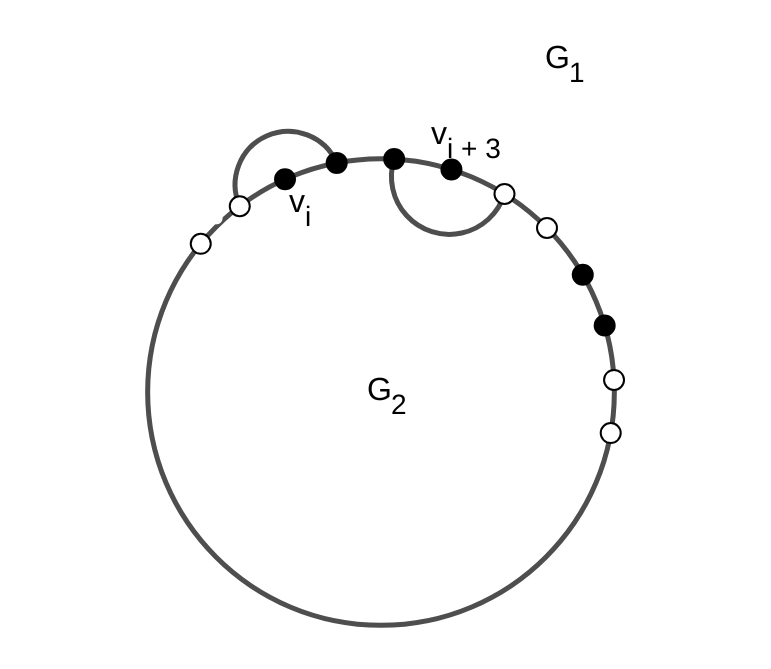
\includegraphics[width=60mm]{hamilton}
    \caption{Coloring a Hamiltonian graph}
    \label{fig:ham}
  \end{figure}
\end{proof}

\begin{remark}
  Whitney \cite{ham1} proved that each triangulated planar graph without separating
  triangles is Hamiltonian. Helden \cite{ham5} strengthened this statement by proving that
  each triangulated planar graph with at most five separating triangles is Hamiltonian.
\end{remark}

With the help of these theorems,
we can also say something about graphs with another kind of $2$-factors.

\begin{claim}
  Let $G$ be a simple triangulated graph of order $n \ge 4$. If $G$ has a $2$-factor
  with none of its cycles having length congruent to $2$ modulo $4$, then the total
  dominating number of $G$ is at least $2$.
\end{claim}

\begin{proof}
  If the $2$-factor consists only of one cycle, then Theorem \ref{thm:ham} proves the
  claim. Suppose that there are at least two cycles in the $2$-factor. First note that
  by alternating colors in pairs, any cycle of length not congruent to $2$ modulo $4$
  can be colored in a way, such that there is at most one vertex with a monochromatic neighborhood.
  (See Figures \ref{fig:4k+1}, \ref{fig:4k+3}.)

  Contract each cycle to a single vertex. $G$ is connected, hence there exists a tree $T$
  in the contracted graph. Choose $T$ to have a minimal number of degree $1$ vertices.
  Let $E(T)$ denote the edges of the original graph that were mapped
  to $T$. We show a $2$-coupon coloring in the subgraph defined by the union of the $2$-factor
  and $E(T)$. Choose a root node $r$ from the degree $1$ vertices in $T$.

  We color the cycle $C_0$
  corresponding to $r$ first. Choose a vertex $v$ in $C_0$, such that there exists a
  $uv$ edge in $E(T)$. We color $C_0$ such that only $v$ may have a monochromatic
  neighborhood and assign $u$ the missing color.

  After this, we iteratively
  color a child of a cycle that is already colored.
  We start by coloring cycles that do not
  correspond to leaves in $T$. Suppose that $C_1$ is a cycle like that, let $C_2$
  be a child of $C_1$, and $v_1v_2$
  be the edge in $E(T)$ such that $v_1 \in C_1$ and $v_2 \in C_2$. Let $c_1$ be a coloring of
  $C_1$ such that only $v_1$ may have a monochromatic neighborhood. There might be
  a vertex (but only one) in $C_1$ that already has a color, so flip the colors of $c_1$ if
  necessary. Color $v_2$ in a way that provides $v_1$ the missing color.

  Now we
  color cycles that correspond to leaves, but have at least $4$ vertices. Let $C_l$ be a
  cycle like that. By Theorem \ref{thm:outerplanar} there
  exists a $2$-coupon coloring $c_l$ of $C_l$. Again, if there is a vertex in $C_l$ that
  already has a color, then we might need to flip the colors of $c_l$.

  Finally, we need to
  color cycles corresponding to leaves of $T$ and having only $3$ vertices. Let $u_lv_lw_l$ be
  a cycle like that, where $v_l$ is the only vertex that may already have a color. Suppose it
  is colored to black. There exists a face $v_lw_lx_l$ where $x_l \neq u_l$.
  If $x_l$ is colored to black, then color $w_l$ and $u_l$ to white. If $x_l$ is colored
  to white, then color $w_l$ to white, and $u_l$ to black. The only remaining case is
  when $x_l$ does not have a color yet. In this case, there must be a face $x_ly_lz_l$
  corresponding to a leaf of $T$. These two leaves have a closest common ancestor
  $t$. $t$ is of degree at least $2$ in $T$, hence $t \neq r$, so $t$ must have degree
  at least $3$. By adding the edge corresponding to $v_lx_l$ to $T$ and removing
  the first edge of the $tv_l$ path, we would get a tree $T'$, where $T'$ would have
  fewer degree $1$ vertices then $T$ has. This contradicts to the choice of $T$.
\end{proof}

\section{Graphs without low-degree vertices}
In this section we will show that the Goddard-Henning conjecture holds for graphs
without too many low-degree vertices. For proving this, we will use a theorem
about coloring hypergraphs. First, let us introduce the necessary definitions.

\begin{definition}
  Let $H$ be a hypergraph. The incidence graph of $H$ is a bipartite graph with one of
  its classes corresponding to the vertices of $H$, and the other class corresponding to
  the hyperedges of $H$. $ve$ is an edge in the incidence graph if and only if the
  hyperedge $e$ contains vertex $v$ in $H$.
\end{definition}
\begin{definition}
  A hypergraph is called planar, if its incidence graph is planar.
\end{definition}
\begin{definition}
  A vertex coloring of a hypergraph is proper if all its hyperedges contain vertices
  from both color classes.
\end{definition}

The following theorem is from Zdenek Dvorák, Daniel Král \cite{hypergraph}.

\begin{thm} \label{thm:hyper}
  Let $H = (V, E)$ be a planar hypergraph with at most $2$ hyperedges of size $2$. Then $H$ has
  a proper vertex coloring with two colors.
\end{thm}
\begin{proof}
  We may assume that $H$ has exactly $2$ hyperedges of size $2$. Otherwise add
  one or two new hyperedges of size $2$. A proper coloring of the resulting hypergraph
  is also a proper coloring of the original one.

  We define another planar graph based on the incidence graph of $H$ as follows.
  For each hyperedge $e$, delete the corresponding vertex from the graph, and
  add edges between the vertices contained in $e$ in a way that it results in a circle.
  The bounded faces of the resulting graph $G_H=(V, F)$ correspond to the hyperedges of $H$.
  (See Figure \ref{fig:hyper}.) After this, triangulate the faces that have more than
  $3$ vertices.

  \begin{figure}[h]
    \centering
    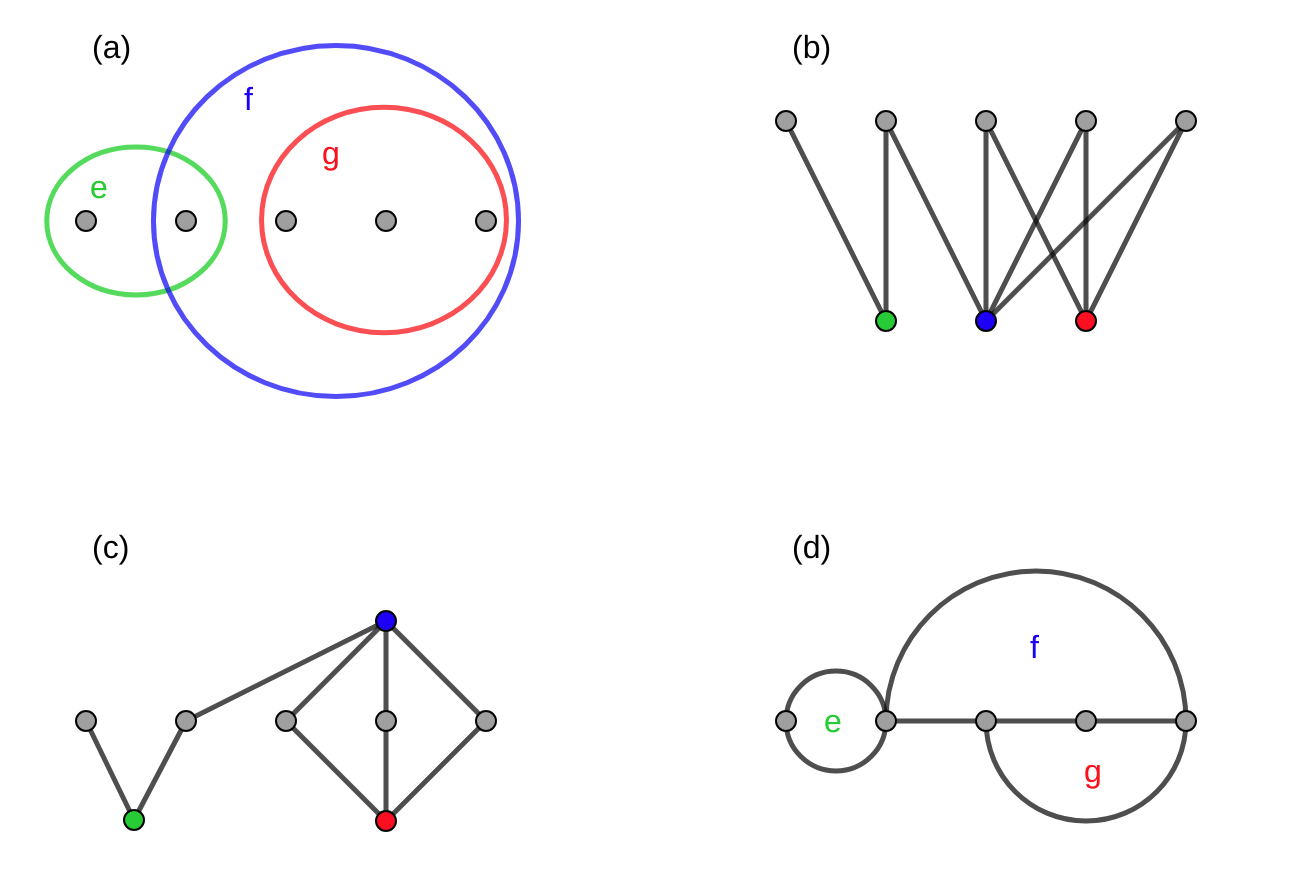
\includegraphics[width=150mm]{hypergraph}
    \caption{A hypergraph (a), its incidence graph (b), a planar embedding of the
      incidence graph (c) and the graph $G_H$ (d)}
    \label{fig:hyper}
  \end{figure}

  Let $c_4$ be a proper $4$-coloring of the resulting graph with colors $\{1, 2, 3, 4\}$.
  By permuting the color classes if necessary, we may assume the followings.
  \begin{enumerate}
    \item If the two hyperedges of size $2$ are not disjoint, i.e. they are $\{u, v\}$ and
      $\{u, w\}$, then $c_4(u) = 1$, and $c_4(v), c_4(w) \in \{3, 4\}$.
    \item If the two hyperedges of size $2$ are disjoint, i.e. they are $\{u, v\}$ and
      $\{x, y\}$, then $c_4(u), c_4(x) \in \{1, 2\}$ and $c_4(v), c_4(y) \in \{3, 4\}$.
  \end{enumerate}
  We define a $2$-coloring of $G_H$ as follows.
  \[
    c_2(v) = \begin{cases}
      1, & \text{if}\ c_4(v) = 1 \ \text{or}\ c_4(v) = 2\\
      2, & \text{if}\ c_4(v) = 3 \ \text{or}\ c_4(v) = 4\\
    \end{cases}
  \]
  We claim that $c_2$ is a proper $2$-coloring of $H$. The hyperedges of size $2$
  have vertices in both color classes due to our assumptions on $c_4$. For the other
  hyperedges there exists a face in $G$ containing the vertices of the hyperedge.
  As $c_4$ was a proper $4$-coloring of the triangulated graph, each face of $G$
  of size at least $3$ has vertices from $3$ or $4$ color classes.
\end{proof}

Now we are ready to prove our claim about graphs without too many low-degree vertices.

\begin{claim}
  Let $G$ be a simple triangulated graph. If there are at most two vertices of degree
  at most $4$, then $G$ has a $2$-coupon coloring.
\end{claim}
\begin{proof}
  By Claim \ref{c:dual} the dual $G^*$ is a $3$-regular $2$-edge-connected planar graph.
  Thus, by Petersen's theorem there exists a perfect matching $M$ in $G^*$. By deleting
  the edges corresponding to $M$ from $G$, we get a graph $G'$ such that all its faces contains
  $4$ vertices. We call such graphs quadrangulated. Note, that for each vertex $v$,
  we deleted at most half of the vertices starting from $v$, thus there are at most
  two vertices in $G'$ of degree $2$ and none of the vertices has less than $2$ neighbors.

  By Lemma \ref{l:bipartite}, $G'$
  is a bipartite graph. Let $U$ and $V$ be the two classes of $G'$. $G'$ is the incidence
  graph of two hypergraphs: let $H_1$ be the hypergraph defined on the vertex set
  $U$ with hyperedges $V$, and $H_2$ be the hypergraph defined on the vertex set $V$
  with hyperedges $U$. By Theorem \ref{thm:hyper}, $H_1$ and $H_2$ has proper $2$-colorings.
  Take the union of these colorings $c$. I.e. on the vertices of $U$, $c$ is defined
  by a proper coloring of $H_1$, whereas on the vertices of $V$, $c$ is defined
  by a proper coloring of $H_2$. $c$ is a $2$-coupon coloring of $G'$.
\end{proof}

\begin{remark}
  It is not true that every simple quadrangulated graph has a $2$-coupon coloring.
  See Figure \ref{fig:quad} for an example.
\end{remark}
\begin{figure}[h]
  \centering
  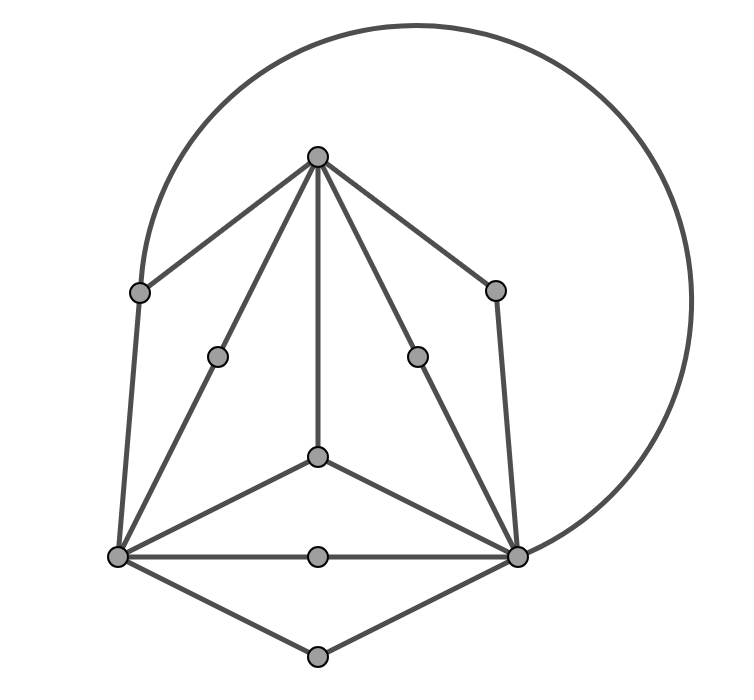
\includegraphics[width=60mm]{quad}
  \caption{A quadrangulated graph without two disjoint dominating sets}
  \label{fig:quad}
\end{figure}

Goddard and Henning \cite{gh} conjectured the following stronger statement about
planar triangulations without degree $3$ vertices.

\begin{conj}
  If $G$ is a simple triangulated graph with all its vertices having degree at least
  $4$, then $G$ admits three disjoint total dominating sets.
\end{conj}

It is also worth noting that having total dominating number at least $2$ can be
translated into a statement about the so-called neighborhood hypergraph. The neighborhood
hypergraph of $G$ is a hypergraph defined on the vertex set of $G$, where for each vertex
$v$, there is a hyperedge containing the neighboring vertices of $v$. $G$ has total
dominating number at least $2$ if and only if the neighborhood hypergraph has a
proper $2$-coloring. In other words,
it is equivalent to the statement that the hyperedges possess property $B$. Its relevance
is that property $B$ has been studied extensively.

\section{Barnette's conjecture}

A conjecture of Barnette \cite{barnette} is the following.
\begin{conj}
  Every $3$-connected cubic planar bipartite graph is Hamiltonian.
\end{conj}

By \ref{ham_dual} if the Barnette-conjecture holds, then the Goddard-Henning
conjecture also holds for Eulerian triangulations.

Alt, Payne, Schmidt and Wood \cite{spec_barnette} proved that the conjecture holds
for graphs, where the dual is an Eulerian planar triangulation and has a special $3$-coloring.

TODO
